\section{\LaTeX-tricks}

In this section we explain some \LaTeX-tricks we use.

\subsection{Figures} 

We include figures by means of \texttt{\textbackslash begin\{figure\}}. Please add a caption and a label to all figures in a unique fashion. The usual width of a figure is $0.85$ times the \texttt{\textbackslash textwidth}.

Refs to figures are done with the \texttt{\textbackslash autoref} package. For referring to a figure with label \texttt{fig:test1} type \texttt{autoref\{fig:test1\}}. The autoref package add the figure keyword without any additional user interaction. Note that also additional keywords, e.g. Table, are supported.

The reference to \autoref{fig:gui} looks like this.

\begin{figure}[h]
	\centering
	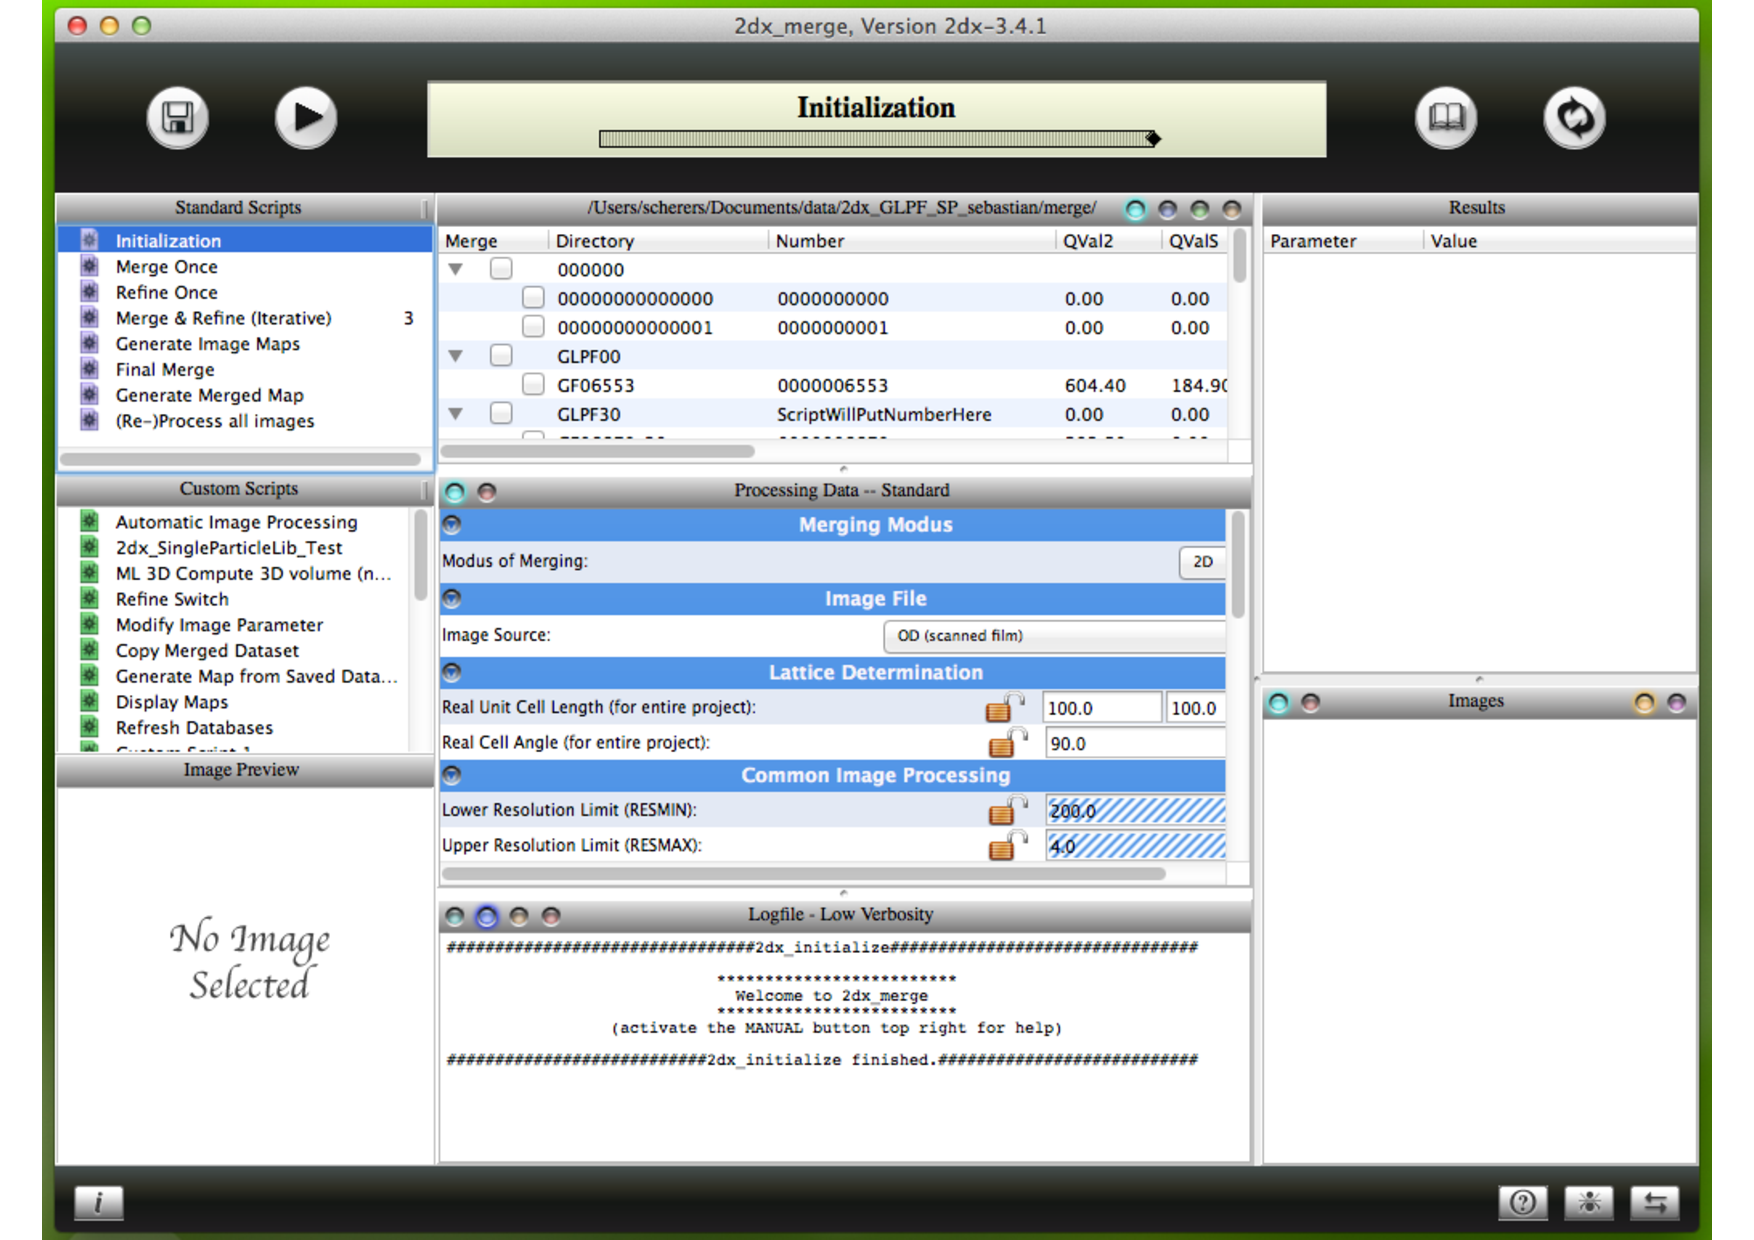
\includegraphics[width=.85\textwidth]{test1.pdf}
	\caption{{\twodx} Gui}
	\label{fig:gui}
\end{figure}

\subsection{Citations}

All sources have to be in the file called "2dx\_manual.bib". As usual we cite them by means of \texttt{\textbackslash cite}. The only deference is that we automatically use the backref package with a fancy style in order to add the back-link in the reference list. A citation looks like this: \cite{Test}.

\subsection{Fancy looking 2dx in the text}
Instead of typing 2dx you should type \texttt{\{\textbackslash twodx\}}. This will paste 2dx in specially looking letters: {\twodx}.

\subsection{Index}
In the end of the manual we have an automatically generated index. All the entries are defined in the text by adding \texttt{\textbackslash index\{Indexentry\}}. For testing we added \texttt{\textbackslash index\{Test Index\}} \textit{here} \index{Test index} in the source code. 

\subsection{Tabulars}
This is a tabular

\vspace{1em}
\begin{tabular}{l l}
		\toprule
		Points & Details \\
		\cmidrule{1-2}
			first point & adsf asf asdfsadffsd fds fjksdfhks ahdfds fdsf sadfaksfs \\
			second point & afsad fsdkfhjsdkjfhkjsdfhskdfhjsd kfhdskj hkjfhklsdjf \\
			third point & sajfkh sdklfh sdf klsdfhjsdklj haslkfjh saldfk asdljfhad \\
		\bottomrule
\end{tabular}\\

\subsection{Conventions}

\begin{description}
\item[Parameters] The name and values of parameters used in {\twodx} should be \textit{italic} so use \texttt{\textbackslash textit}. They also should be part of the Index.
\item[Names] Any names such as the name of GUI panel should be "quoted".
\item[Programs] If a program is mentioned in the text it should be marked with  \texttt{\textbackslash textit} like this \textit{2dx\_getlattice}. The MRC programs can be capitalized to distinguish them from the others. And citing the author should also be done.
\end{description}


